% Options for packages loaded elsewhere
\PassOptionsToPackage{unicode}{hyperref}
\PassOptionsToPackage{hyphens}{url}
\documentclass[
  ignorenonframetext,
]{beamer}
\newif\ifbibliography
\usepackage{pgfpages}
\setbeamertemplate{caption}[numbered]
\setbeamertemplate{caption label separator}{: }
\setbeamercolor{caption name}{fg=normal text.fg}
\beamertemplatenavigationsymbolsempty
% remove section numbering
\setbeamertemplate{part page}{
  \centering
  \begin{beamercolorbox}[sep=16pt,center]{part title}
    \usebeamerfont{part title}\insertpart\par
  \end{beamercolorbox}
}
\setbeamertemplate{section page}{
  \centering
  \begin{beamercolorbox}[sep=12pt,center]{section title}
    \usebeamerfont{section title}\insertsection\par
  \end{beamercolorbox}
}
\setbeamertemplate{subsection page}{
  \centering
  \begin{beamercolorbox}[sep=8pt,center]{subsection title}
    \usebeamerfont{subsection title}\insertsubsection\par
  \end{beamercolorbox}
}
% Prevent slide breaks in the middle of a paragraph
\widowpenalties 1 10000
\raggedbottom
\AtBeginPart{
  \frame{\partpage}
}
\AtBeginSection{
  \ifbibliography
  \else
    \frame{\sectionpage}
  \fi
}
\AtBeginSubsection{
  \frame{\subsectionpage}
}
\usepackage{iftex}
\ifPDFTeX
  \usepackage[T1]{fontenc}
  \usepackage[utf8]{inputenc}
  \usepackage{textcomp} % provide euro and other symbols
\else % if luatex or xetex
  \usepackage{unicode-math} % this also loads fontspec
  \defaultfontfeatures{Scale=MatchLowercase}
  \defaultfontfeatures[\rmfamily]{Ligatures=TeX,Scale=1}
\fi
\usepackage{lmodern}
\ifPDFTeX\else
  % xetex/luatex font selection
\fi
% Use upquote if available, for straight quotes in verbatim environments
\IfFileExists{upquote.sty}{\usepackage{upquote}}{}
\IfFileExists{microtype.sty}{% use microtype if available
  \usepackage[]{microtype}
  \UseMicrotypeSet[protrusion]{basicmath} % disable protrusion for tt fonts
}{}
\makeatletter
\@ifundefined{KOMAClassName}{% if non-KOMA class
  \IfFileExists{parskip.sty}{%
    \usepackage{parskip}
  }{% else
    \setlength{\parindent}{0pt}
    \setlength{\parskip}{6pt plus 2pt minus 1pt}}
}{% if KOMA class
  \KOMAoptions{parskip=half}}
\makeatother
\usepackage{longtable,booktabs,array}
\newcounter{none} % for unnumbered tables
\usepackage{calc} % for calculating minipage widths
\usepackage{caption}
% Make caption package work with longtable
\makeatletter
\def\fnum@table{\tablename~\thetable}
\makeatother
\usepackage{graphicx}
\makeatletter
\newsavebox\pandoc@box
\newcommand*\pandocbounded[1]{% scales image to fit in text height/width
  \sbox\pandoc@box{#1}%
  \Gscale@div\@tempa{\textheight}{\dimexpr\ht\pandoc@box+\dp\pandoc@box\relax}%
  \Gscale@div\@tempb{\linewidth}{\wd\pandoc@box}%
  \ifdim\@tempb\p@<\@tempa\p@\let\@tempa\@tempb\fi% select the smaller of both
  \ifdim\@tempa\p@<\p@\scalebox{\@tempa}{\usebox\pandoc@box}%
  \else\usebox{\pandoc@box}%
  \fi%
}
% Set default figure placement to htbp
\def\fps@figure{htbp}
\makeatother
\setlength{\emergencystretch}{3em} % prevent overfull lines
\providecommand{\tightlist}{%
  \setlength{\itemsep}{0pt}\setlength{\parskip}{0pt}}
% Slide layout defaults for warning-clean scientific decks.
\usepackage{etoolbox}
\IfFileExists{xurl.sty}{\usepackage{xurl}}{}
\IfFileExists{seqsplit.sty}{\usepackage{seqsplit}}{\newcommand{\seqsplit}[1]{#1}}
\protected\def\breakseq#1{\seqsplit{#1}}
\protected\def\breaktt#1{\begingroup\ttfamily\seqsplit{#1}\endgroup}
\setlength{\emergencystretch}{6em}
\tolerance=5000
\hbadness=10000
\hfuzz=1pt
\setlength{\tabcolsep}{2pt}
\AtBeginEnvironment{longtable}{\tiny\renewcommand{\arraystretch}{0.86}\setlength{\tabcolsep}{1pt}}
\AtBeginEnvironment{tabular}{\tiny\renewcommand{\arraystretch}{0.86}\setlength{\tabcolsep}{1pt}}

% Natbib and cross-reference fallbacks — slides don't load natbib
% or cleveref, but combined-PDF manuscript prose may emit these
% commands. The fallback renders citations as a bracketed key list
% and cross-references as detokenized labels so slides don't fail on
% undefined control sequences or raw underscores. \providecommand is
% a no-op if packages load later.
\providecommand{\citep}[1]{[#1]}
\providecommand{\citet}[1]{#1}
\providecommand{\citealp}[1]{#1}
\providecommand{\citeauthor}[1]{#1}
\providecommand{\citeyear}[1]{#1}
\providecommand{\cref}[1]{\texttt{\detokenize{#1}}}
\providecommand{\Cref}[1]{\texttt{\detokenize{#1}}}

\newtheorem{proposition}{Proposition}
\newtheorem{hypothesis}{Hypothesis}
\usepackage{bookmark}
\IfFileExists{xurl.sty}{\usepackage{xurl}}{} % add URL line breaks if available
\urlstyle{same}
% fallback for those not using the hyperref driver hyperxmp:
\makeatletter
\@ifundefined{xmpquote}{\newcommand{\xmpquote}[1]{#1}}{}
\makeatother
\hypersetup{
  hidelinks,
  pdfcreator={LaTeX via pandoc}}

\author{\texorpdfstring{}{}}
\date{}

\begin{document}

\section{Integration: Unified Pipeline and Token
Injection}\label{sec:integration}

\begin{frame}[fragile,allowframebreaks]{Architecture Overview}
\protect\phantomsection\label{architecture-overview}
The three resource layers described in @sec:pools, @sec:rules, and
@sec:tools are orchestrated by a single function in
\breaktt{src/integration.py}. The \breaktt{run\_integration\_demo()}
function calls all three subsystems in a defined order, collects their
results into a structured dictionary, and writes summary counts to
\breaktt{output/data/manuscript\_variables.json} for injection into this
manuscript at render time. @fig:architecture illustrates the complete
architecture.

\begin{verbatim}
run_integration_demo()
  ├── read_bibliography_fond()       → {"manifest": ..., "bibtex": ..., "csv_rows": [...]}
  ├── read_contacts_fond()           → {"manifest": ..., "contacts": [...]}
  ├── read_datasets_fond()           → {"manifest": ..., "datasets": [...]}
  ├── validate_against_rules("template_project_rules")    → {"status": "ok", ...}
  ├── validate_against_rules("template_manuscript_rules") → {"status": "ok", ...}
  ├── discover_tools()               → [{"name": ..., "manifest": ...}, ...]
  └── validate_tool_scripts_exist(<each tool>)            → {"status": "ok", ...}
\end{verbatim}

The function returns a top-level dict with keys \texttt{fonds},
\texttt{rules}, \texttt{tools}, and \texttt{summary}. The
\texttt{summary} sub-dict provides the counts that populate manuscript
tokens.
\end{frame}

\begin{frame}[fragile,allowframebreaks]{Manuscript Variable Tokens}
\protect\phantomsection\label{manuscript-variable-tokens}
The token injection system bridges the integration pipeline and the
manuscript prose. Tokens use double-brace syntax: \texttt{3} expands to
the integer count of fonds successfully loaded during the most recent
integration run. Tokens are resolved by
\breaktt{scripts/03\_generate\_manuscript.py}, which reads
\breaktt{output/data/manuscript\_variables.json} and substitutes each
token before the manuscript is passed to the rendering engine.

\begin{figure}
\centering
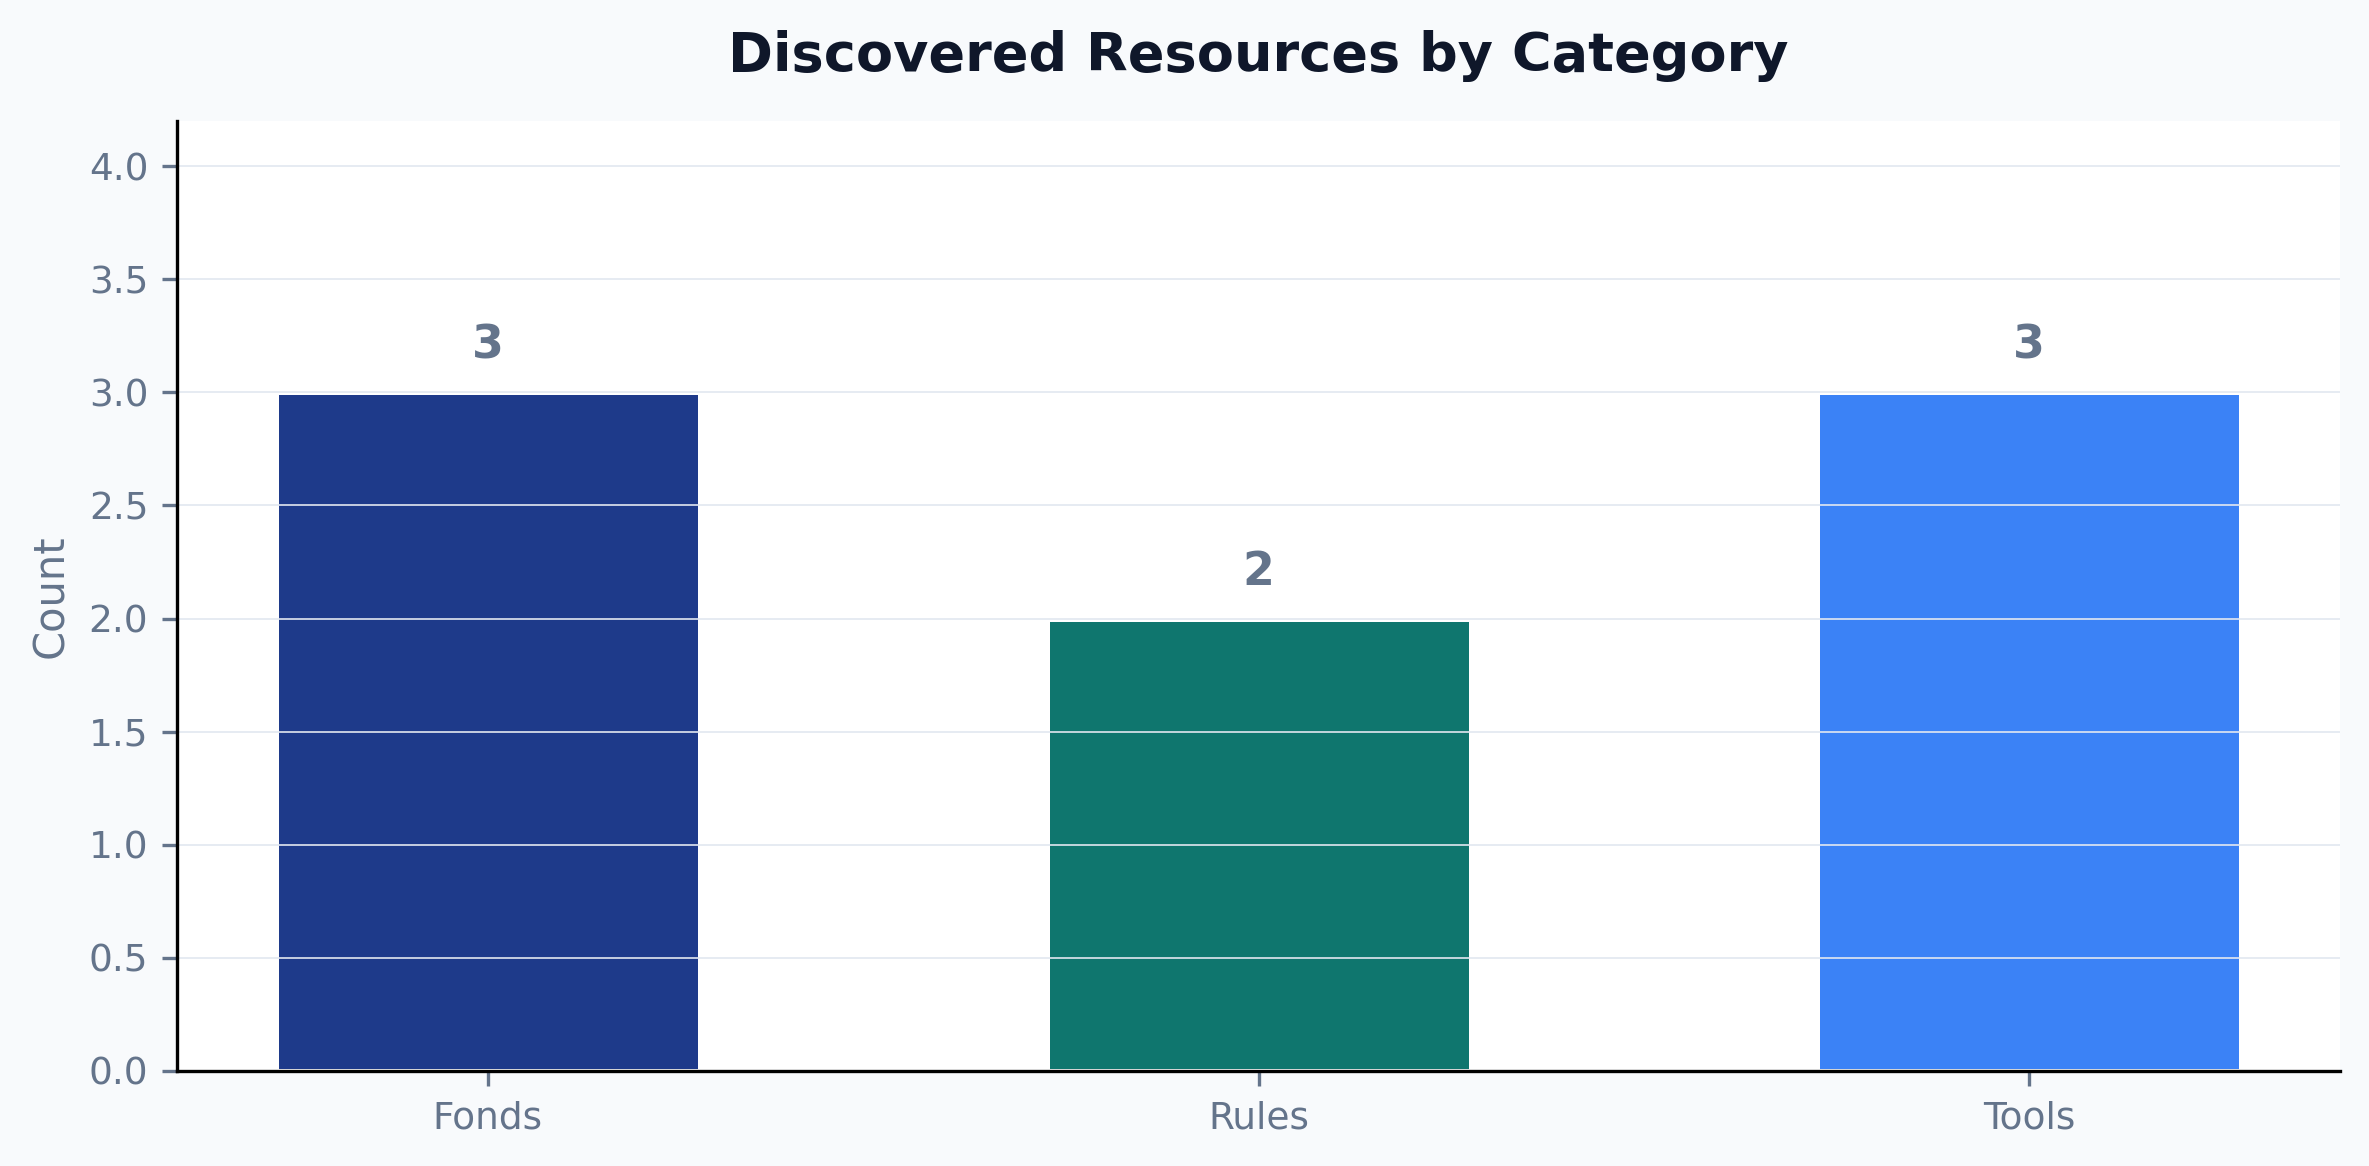
\includegraphics[width=0.75\linewidth,height=0.46\textheight,keepaspectratio,alt={Runtime integration counts from manuscript\_variables.json. Bars show fonds loaded, rule sets validated, and tools discovered during a single pipeline run.}]{../figures/resource_counts.png}
\caption{Runtime integration counts from manuscript\_variables.json.
Bars show fonds loaded, rule sets validated, and tools discovered during
a single pipeline run.}\label{fig:counts}
\end{figure}

The current \breaktt{manuscript\_variables.json} contains the following
summary values (see @fig:counts for a visual representation):

{\def\LTcaptype{none} % do not increment counter
\begin{longtable}[]{@{}ll@{}}
\toprule\noalign{}
Token & Value \\
\midrule\noalign{}
\endhead
\texttt{3} & 3 \\
\texttt{2} & 2 \\
\texttt{3} & 3 \\
\texttt{8} & 8 \\
\bottomrule\noalign{}
\end{longtable}
}

This table is itself token-injected: the values shown are those produced
by the pipeline, not hard-coded by the manuscript author. If the
pipeline results change --- for example, because a new fond is added ---
re-running \breaktt{scripts/03\_generate\_manuscript.py} updates the
manuscript automatically, without manual editing. This property is
central to reproducibility: the manuscript's quantitative claims are
always consistent with the code that generated them
\breakseq{[@Stodden2016enhancing]}.
\end{frame}

\begin{frame}[fragile,allowframebreaks]{Methods: The Script Pipeline}
\protect\phantomsection\label{methods-the-script-pipeline}
Six thin orchestration scripts govern the integration workflow
(@fig:pipeline, @fig:pipelineflow):

{\def\LTcaptype{none} % do not increment counter
\begin{longtable}[]{@{}
  >{\raggedright\arraybackslash}p{(\linewidth - 4\tabcolsep) * \real{0.3333}}
  >{\raggedright\arraybackslash}p{(\linewidth - 4\tabcolsep) * \real{0.3333}}
  >{\raggedright\arraybackslash}p{(\linewidth - 4\tabcolsep) * \real{0.3333}}@{}}
\toprule\noalign{}
\begin{minipage}[b]{\linewidth}\raggedright
Script
\end{minipage} & \begin{minipage}[b]{\linewidth}\raggedright
Purpose
\end{minipage} & \begin{minipage}[b]{\linewidth}\raggedright
Key output
\end{minipage} \\
\midrule\noalign{}
\endhead
\breaktt{scripts/01\_validate\_sources.py} & Validate presence and
well-formedness of all resources & Console report \\
\breaktt{scripts/02\_run\_integration.py} & Run
\breaktt{run\_integration\_demo()} and print JSON summary & Console
JSON \\
\breaktt{scripts/03\_generate\_manuscript.py} & Write
\breaktt{output/data/manuscript\_variables.json} & JSON file \\
\breaktt{scripts/04\_validate\_strong\_rules.py} & Semantic evaluation of
strong-rule constraints (@sec:rules) against this project's own tree &
Console report, non-zero exit on violation \\
\breaktt{scripts/05\_generate\_figures.py} & Render all 8 content figures
plus the cover illustration & 9 PNG files under
\breaktt{manuscript/figures/} \\
\breaktt{scripts/z\_generate\_manuscript\_variables.py} & Hydrate
\texttt{\{\{TOKEN\}\}} values and inject them into
\breaktt{output/manuscript/} immediately before rendering & JSON file +
resolved manuscript tree \\
\bottomrule\noalign{}
\end{longtable}
}

\begin{figure}
\centering
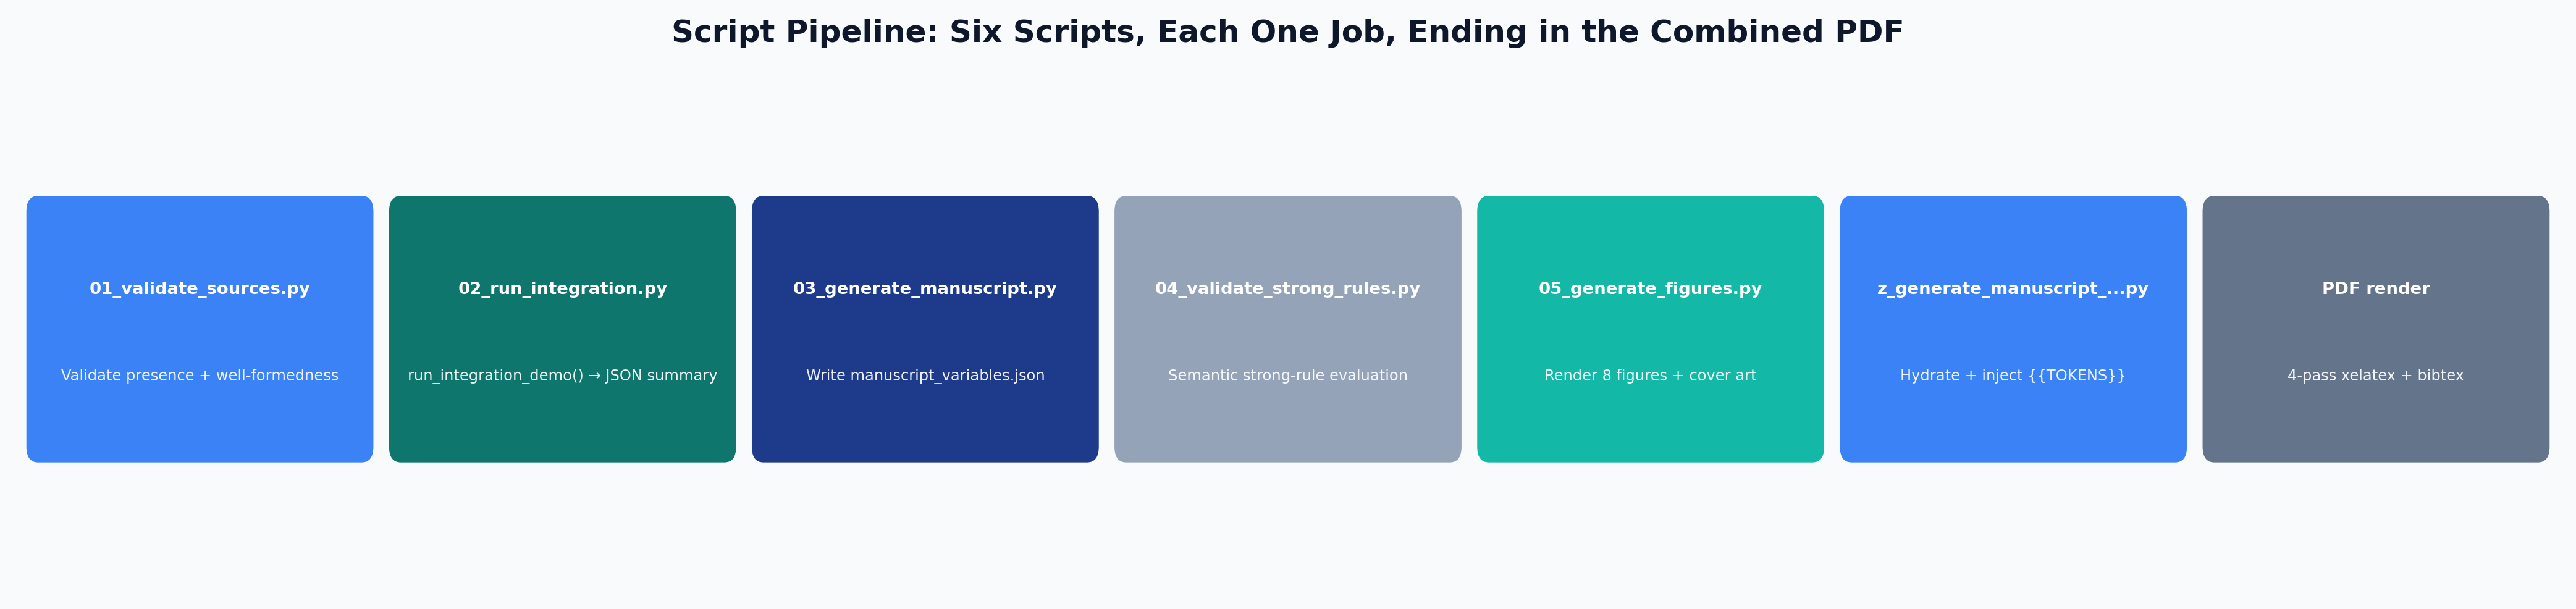
\includegraphics[width=0.95\linewidth,height=0.46\textheight,keepaspectratio,alt={The six-script pipeline from source validation through token hydration, ending at the combined-PDF render step.}]{../figures/pipeline_flow.png}
\caption{The six-script pipeline from source validation through token
hydration, ending at the combined-PDF render
step.}\label{fig:pipelineflow}
\end{figure}

\begin{figure}
\centering
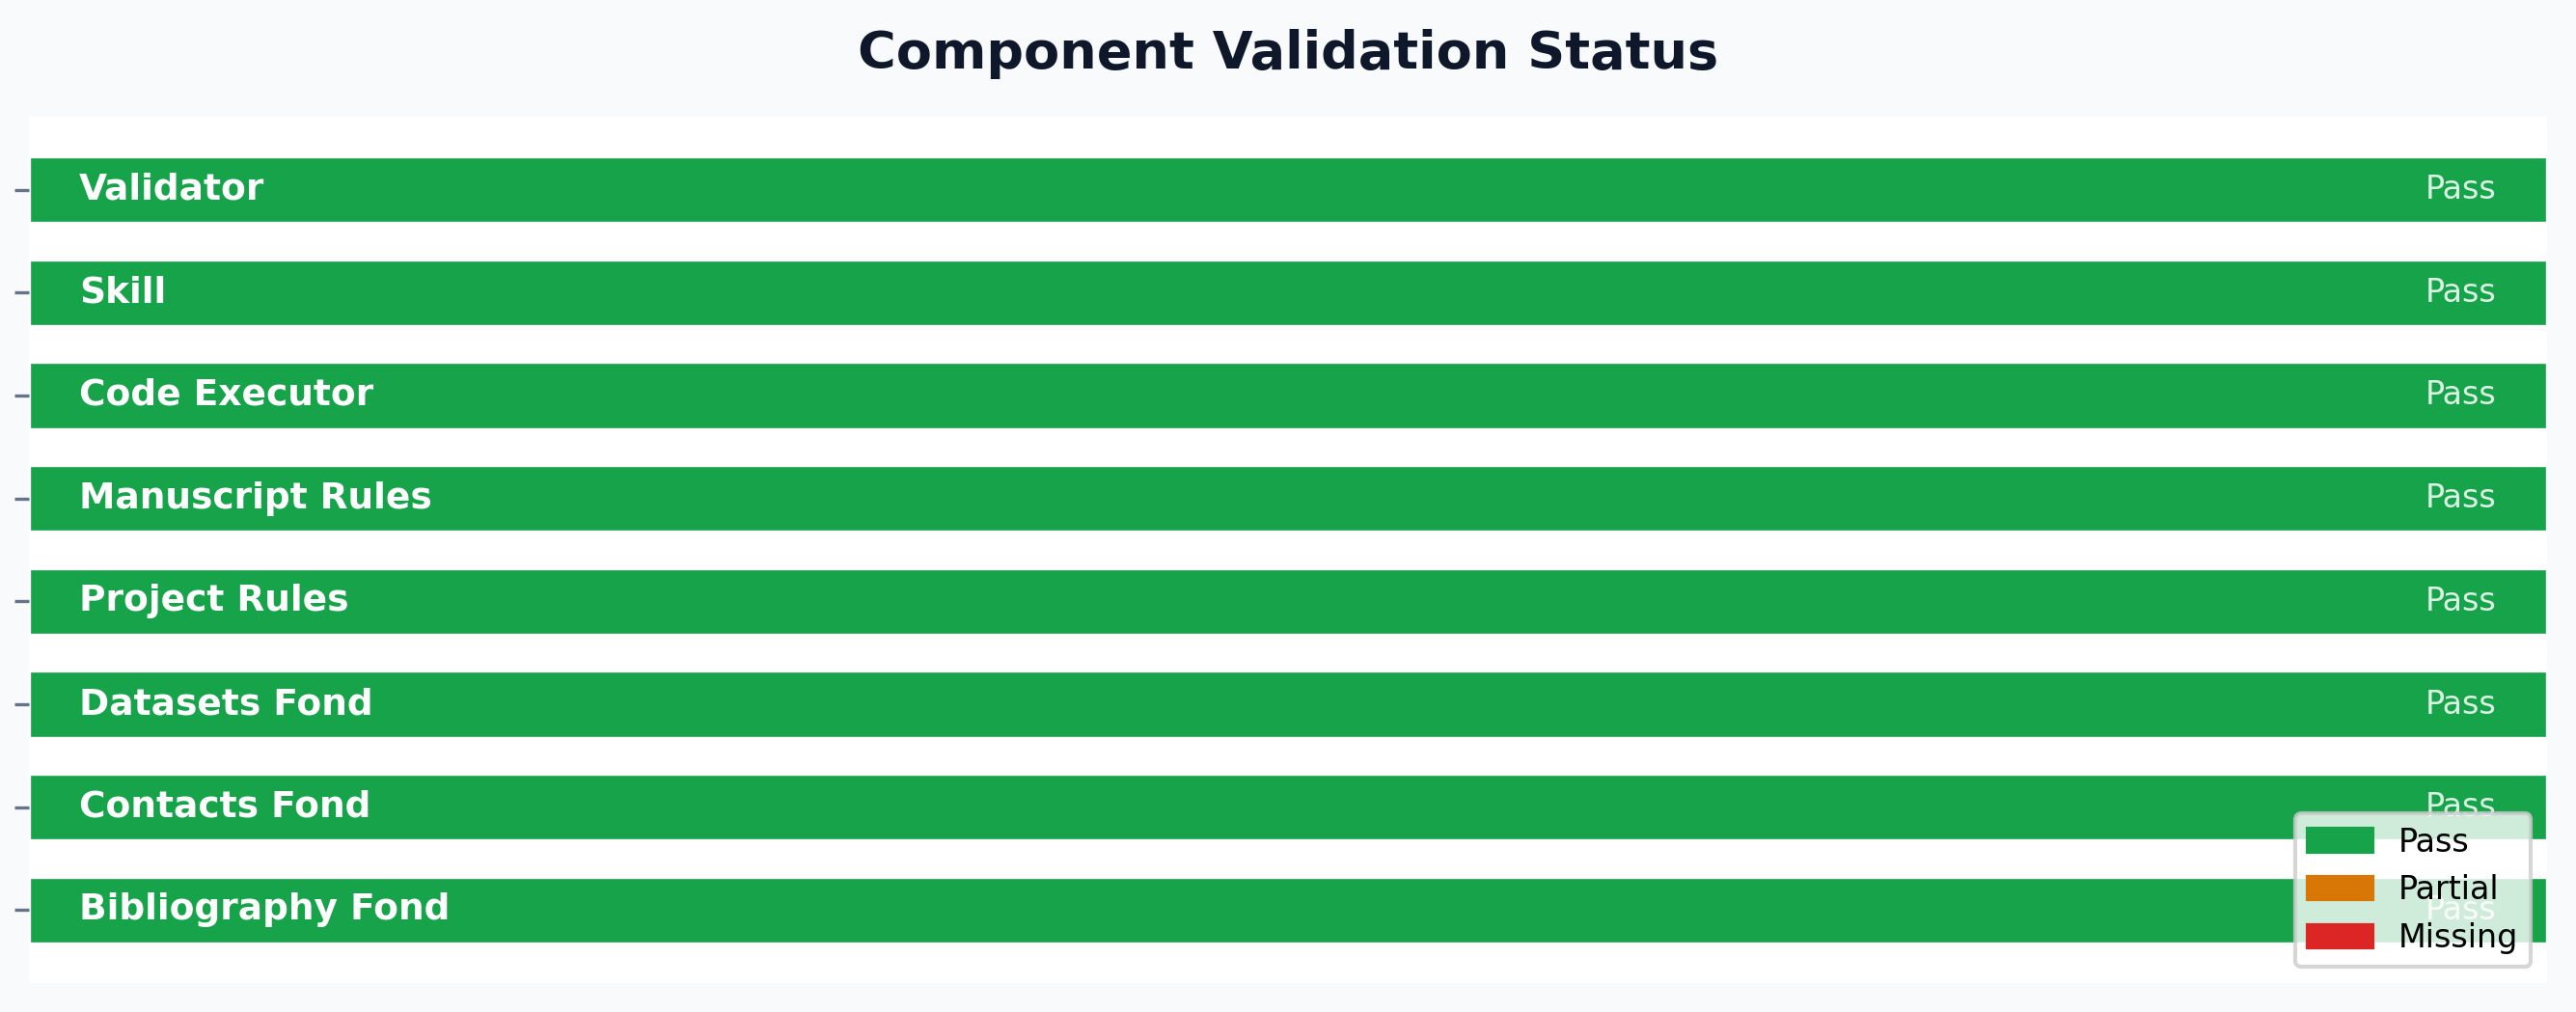
\includegraphics[width=0.85\linewidth,height=0.46\textheight,keepaspectratio,alt={Integration status dashboard showing per-resource validation results. Green indicates ok, amber indicates partial, red indicates missing.}]{../figures/status_dashboard.png}
\caption{Integration status dashboard showing per-resource validation
results. Green indicates ok, amber indicates partial, red indicates
missing.}\label{fig:pipeline}
\end{figure}

@fig:pipelineflow traces this sequence left to right: source validation
feeds the integration demo, whose summary feeds both the
manuscript-variable token file and the strong-rule semantic evaluator;
the figure-generation stage runs independently; and
\breaktt{z\_generate\_manuscript\_variables.py} --- invoked automatically
by the rendering pipeline immediately before the PDF render step --- is
what actually substitutes every \texttt{\{\{TOKEN\}\}} and writes the
resolved manuscript that pandoc consumes. @fig:pipeline shows the
corresponding per-component pass/partial/missing status from the same
run.

Each script imports all business logic from \texttt{src/} and stays free
of computation of its own --- the longest,
\breaktt{01\_validate\_sources.py} at 112 lines, is entirely CLI plumbing
(argument parsing, console formatting) around calls into
\breaktt{src/fonds\_reader.py}, \breaktt{src/rules\_applier.py}, and
\breaktt{src/tools\_invoker.py}. This thin-orchestrator pattern
\breakseq{[@Wilson2014best]} ensures that all testable logic is in
\texttt{src/} at ≥ 90\% coverage, while the scripts themselves remain
readable without a dedicated test suite of their own.
\end{frame}

\begin{frame}[fragile,allowframebreaks]{Resilience Design}
\protect\phantomsection\label{resilience-design}
The integration layer enforces resilience at three levels, corresponding
to the three failure modes a monorepo integration pipeline encounters:

\begin{enumerate}
\item
  \textbf{Resource absence}: A fond, rule set, or tool directory may not
  yet exist if the resource was created by a parallel agent that has not
  yet completed. All three reader modules return \texttt{None} or empty
  collections in this case, and \breaktt{run\_integration\_demo()}
  reports the missing resource in the \texttt{summary} dict without
  raising.
\item
  \textbf{Schema malformation}: A manifest may be present but contain
  invalid YAML or missing required fields. Readers catch
  \texttt{yaml.YAMLError} and return a degraded result
  (\breaktt{status="partial"} in rule validation; \texttt{None} in fond
  reading) rather than propagating the parse error.
\item
  \textbf{Script absence}: A tool may declare entrypoints in its
  manifest that have not yet been created.
  \breaktt{validate\_tool\_scripts\_exist()} detects this at discovery
  time and returns \breaktt{status="partial"} with a list of missing
  script paths, so the pipeline can report the defect without attempting
  to invoke a non-existent script.
\end{enumerate}

\begin{figure}
\centering
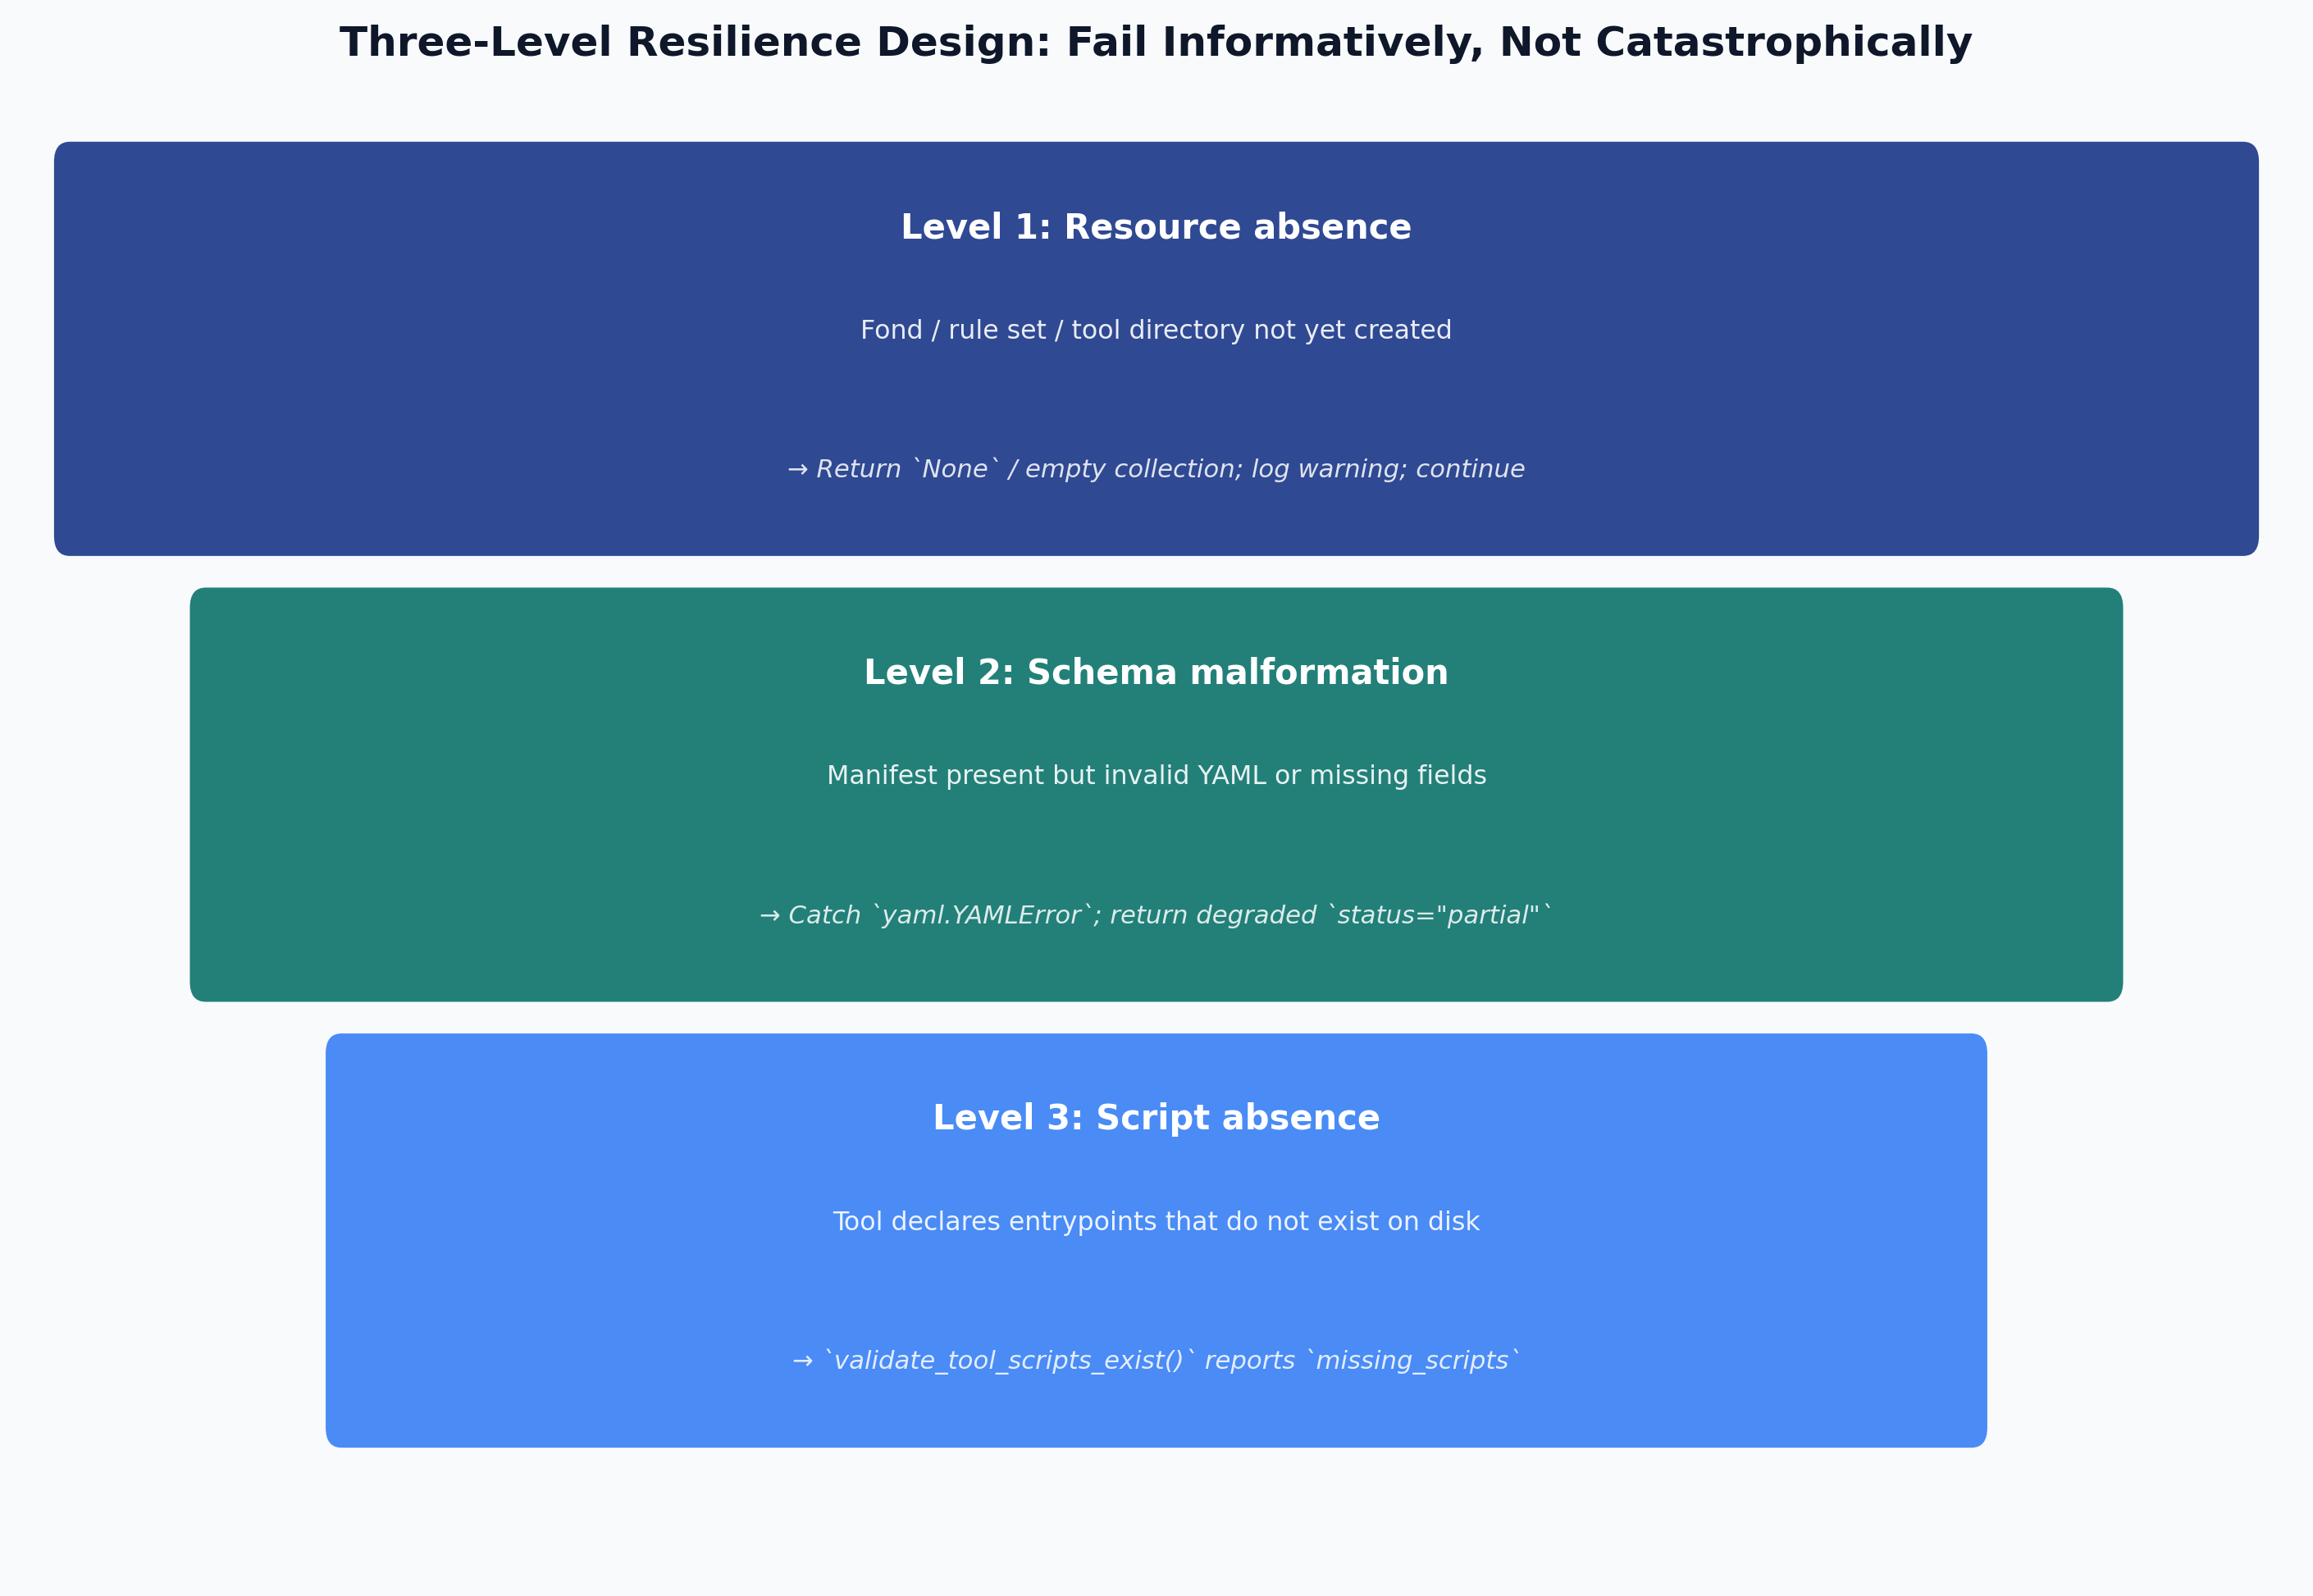
\includegraphics[width=0.85\linewidth,height=0.46\textheight,keepaspectratio,alt={The integration layer's three-level resilience design: resource absence, schema malformation, and script absence, each with its own graceful-degradation response.}]{../figures/resilience_layers.png}
\caption{The integration layer's three-level resilience design: resource
absence, schema malformation, and script absence, each with its own
graceful-degradation response.}\label{fig:resilience}
\end{figure}

This three-level resilience design reflects the principle that
shared-resource pipelines should fail \emph{informatively} rather than
\emph{catastrophically} --- surfacing the cause of incompleteness in
structured output that downstream consumers can act on
\breakseq{[@Taschuk2017ten]}. @fig:resilience presents the three levels as a
single funnel: each level's failure mode and graceful-degradation
response, read top to bottom in the order a pipeline run actually
encounters them (resource discovery happens before schema parsing, which
happens before script-existence checks).
\end{frame}

\begin{frame}[fragile,allowframebreaks]{Performance and Overhead}
\protect\phantomsection\label{performance-and-overhead}
The resilience design above trades a small, constant amount of I/O
overhead for the ability to degrade gracefully. Each reader performs at
most two filesystem existence checks (\breaktt{pathlib.Path.exists()})
before attempting a read, and every YAML parse uses
\breaktt{yaml.safe\_load()} rather than a schema-validating parser ---
the module deliberately performs \emph{structural} validation
(parseable, expected top-level keys present) and leaves deep
\emph{semantic} validation to the dedicated
\breaktt{strong\_rule\_evaluator} module (@sec:rules) rather than paying
that cost on every discovery call. In practice,
\breaktt{scripts/02\_run\_integration.py} completes in well under a
second on the exemplar's small fond/rule/tool counts; the design does
not attempt to optimise for repositories with thousands of fonds, since
the target use case is a curated, human-reviewed set of shared resources
rather than a large-scale data catalogue.
\end{frame}

\begin{frame}[fragile,allowframebreaks]{Test Coverage}
\protect\phantomsection\label{test-coverage}
The eight \texttt{src/} modules --- \texttt{fonds\_reader},
\texttt{rules\_applier}, \texttt{tools\_invoker}, \texttt{integration},
\texttt{figures}, \breaktt{strong\_rule\_evaluator},
\breaktt{manuscript\_variables}, and \texttt{type\_defs} --- are covered
by tests across nine test files in \texttt{tests/}, including
property-based tests (\breaktt{test\_property\_based.py}) and
coverage-extras tests targeting previously-uncovered branches
(\breaktt{test\_coverage\_extras.py}). Tests use real file paths, real
YAML files, and real BibTeX content rather than mocks, ensuring that
coverage numbers reflect genuine code paths through the
resource-discovery logic. The current coverage report shows combined
line coverage comfortably above the project's 90\% floor;
\breaktt{strong\_rule\_evaluator.py}, the newest and most branch-heavy
module, has the most room for additional edge-case tests, while the
remaining seven modules are at or near 100\%. These exact test/coverage
counts drift as the suite grows --- treat the figures above as a
snapshot, not a frozen claim, and re-run
\breaktt{uv\ run\ pytest\ …\ -\/-cov-report=term} for the current
numbers. The \breaktt{tests/test\_integration.py} suite includes an
end-to-end test that calls \breaktt{run\_integration\_demo()} and asserts
that the \texttt{summary} dict contains the expected keys with
non-negative integer values --- a contract test that verifies the token
injection pipeline's data source.
\breaktt{tests/test\_manuscript\_variables.py} adds a negative control:
it monkeypatches \breaktt{run\_integration\_demo()}'s return value and
asserts the derived tokens actually change, proving the token-generation
function is live-wired to its source rather than emitting a hard-coded
constant.
\end{frame}

\end{document}
